%!TEX root = apostila.tex
% \section{Definição}
\label{chap:automacao}
A palavra automação vem do latim \emph{automatus} -- mover por si mesmo. Logo a automação de uma tarefa consiste em fazer com que tal tarefa seja realizada sem envolver trabalho humano. Isto pode ser por diversos motivos: seja por que é uma tarefa perigosa e portanto queremos aumentar a segurança das pessoas, seja para fazer a tarefa de forma mais rápida, seja para melhorar a qualidade do produto final ou seja porque simplesmente o custo do trabalho humano é muito elevado. Logo, podemos definir automação da seguinte forma:
\begin{quote}
  Automação é a substituição do trabalho humano por sistemas autônomos visando melhorar segurança, qualidade, produção e/ou custos.
\end{quote}

Neste contexto, automação industrial é nada mais que a automação de um sistema industrial, ou de um sistema de manufatura. Embora manufatura venha de \emph{fazer com as mãos}, desde a revolução industrial que usamos esta palavra significando simplesmente a fabricação de algum produto. Juntando então o conceito de automação, têm-se:
\begin{quote}
  A automação industrial consiste em implementar os processos necessários para a manufatura de algum produto com o mínimo de esforço humano, físico ou mental, visando melhor segurança, qualidade, produção e/ou custo.
\end{quote}

Com base nesta definição, qualquer sistema que realize a manufatura de algum produto automaticamente e sem usar esforço humano é um sistema automatizado. Logo, uma máquina por mais complexa que seja mas que funcione a manivela, tal como uma calculadora mecânica, não se classifica como automação. Da mesma forma uma máquina que não exija esforço físico mas requeira atenção constante, tal como um carro ou mesmo uma batedeira, também não é automatizada; neste último caso usa-se o termo mecanizada.

Do ponto de vista econômico, a manufatura é a transformação de materiais (matéria prima) em itens de maior valor (produto). Isto é conseguido por uma determinada sequência de processos químicos e físicos. De forma mais sucinta:
\begin{quote}
	Manufatura é a transformação de matéria prima em produtos pela aplicação de um ou mais processos.
\end{quote}

Ou seja, na automação industrial estamos interessados em estudar métodos e ferramentas que permitam deixar os processos de manufatura os mais independentes possível da interferência humana. 

\section{Classificação}

O próprio avanço dos sistemas de automação permite com que se tenham equipamentos cada vez mais versáteis, que não sejam feitos para a fabricação de um único produto. Esta possibilidade de equipamentos versáteis levam a, grosso modo, 3 tipos de automação, tal qual mostra a figura \ref{fig:tipos_automacao}: fixa, flexível e programável. Tipicamente são fatores econômicos que levam a escolha de um destes tipos.

\begin{figure}[hbt]
	\begin{center}
    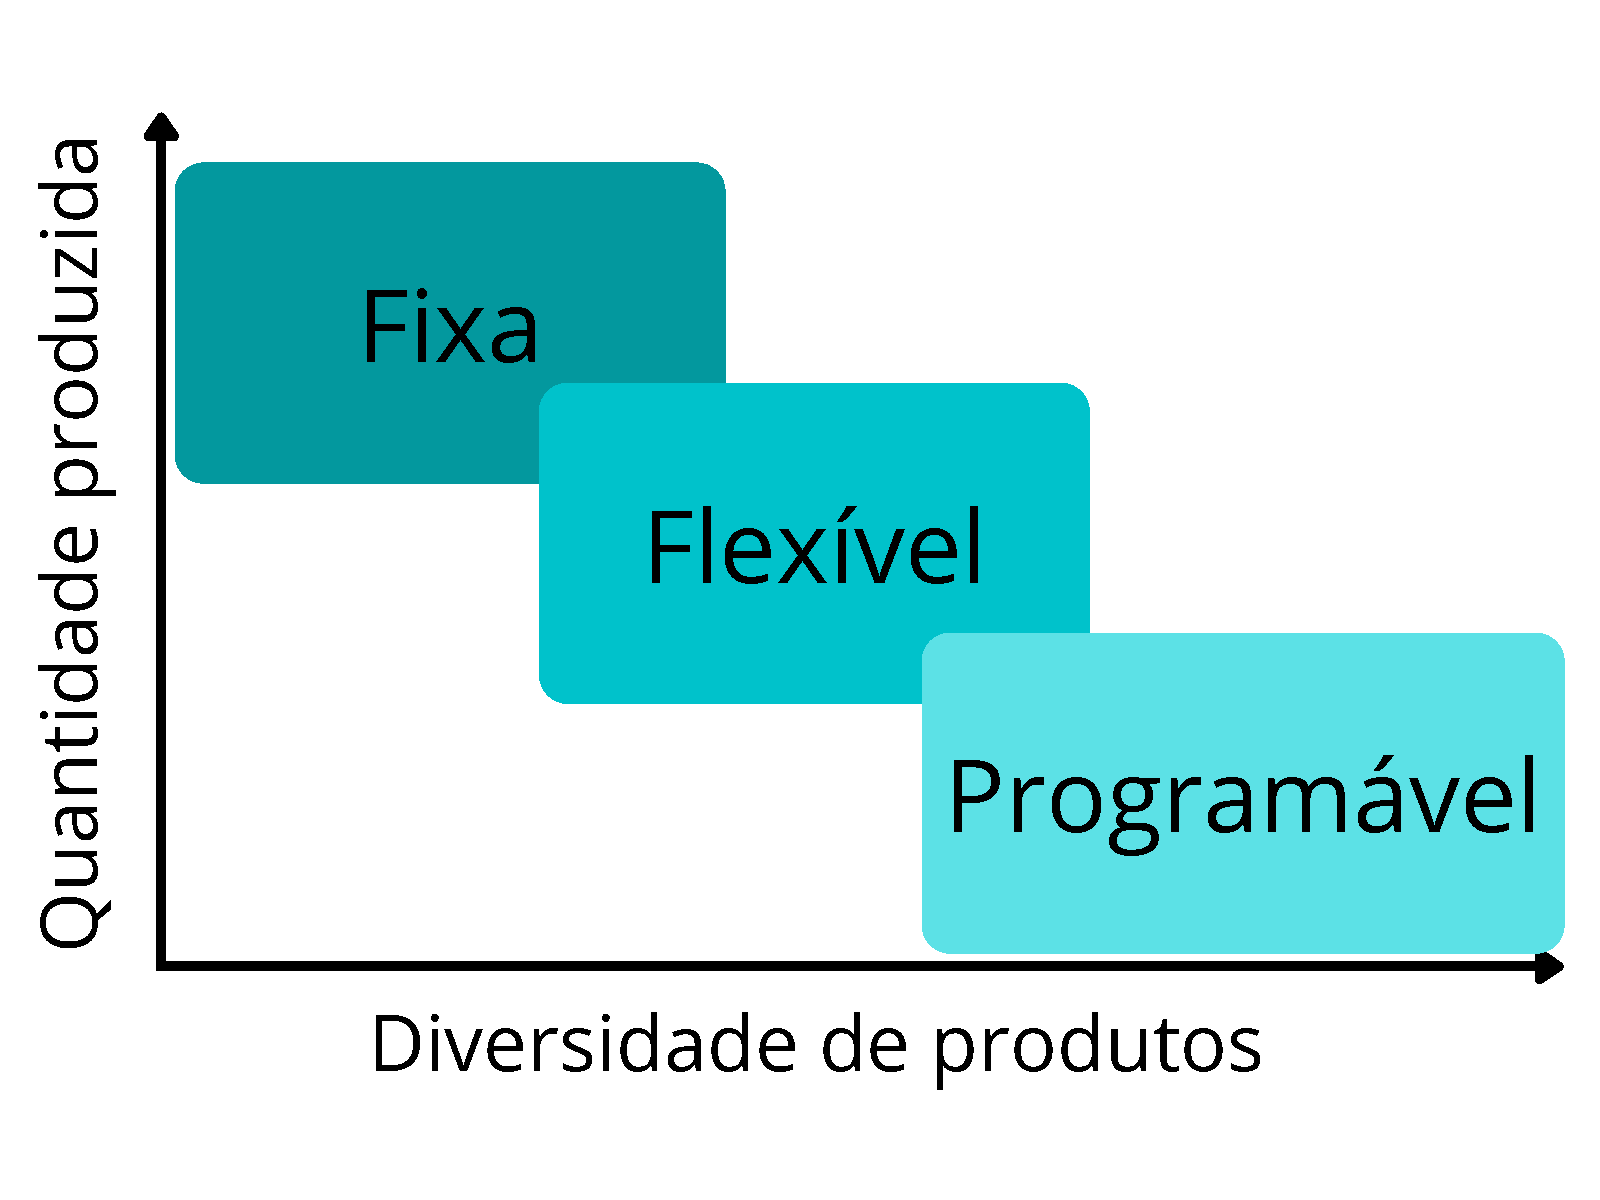
\includegraphics[width=0.8\textwidth  ]{figuras/fixaflexprog}
%		\includegraphics[width=0.6\textwidth]{tipos_automacao}
	% \tikzstyle{area}=[draw,rectangle,rounded corners,text centered,text width=2.2cm,minimum height=1.2cm]
	% \begin{tikzpicture}
	% 	\draw[very thick, ->, >=stealth'](0,0)--(5.5,0);
	% 	\draw(5.5,0)node[below left]{Diversidade};
	% 	\draw[very thick, ->, >=stealth'](0,0)--(0,3.3);
	% 	\draw(0,3.3)node[above left, rotate=90]{Quantidade};
	% 	\draw(1.25,2.5)node[area]{Fixa} (2.5,1.55)node[area]{Flexível} (4,0.6)node[area]{Programável};
	% \end{tikzpicture}
	\end{center}
	\caption{Tipos de automação industrial quanto a quantidade e diversidade de produtos.}
	\label{fig:tipos_automacao}
\end{figure}

A automação fixa é aplicada à produção de um único produto (ou com mínimas variações), em grandes quantidades: refinaria de petróleo, parafuso, tampas de garrafa, clipes de papel, elos de corrente, biscoito, cerveja, etc. Ela utiliza equipamentos feitos sob medida para cada processo, que portanto tem alto custo inicial mas grande produtividade.

A automação flexível é aplicada à produção de produtos parecidos, em que pequenas modificações permitem a alteração do produto, como por exemplo mudança de um perfil a ser prensado ou extrudado ou a mudança das quantidades do mesmo conjunto de matérias primas (mudança de receita). Tipicamente é feita a chamada fabricação em lotes, onde entre um lote e outro se alteram as peças e/ou as sequências a serem seguidas de forma automática para ter o menor tempo parado possível. Exemplos são livros, circuitos integrados, potes de plástico, panelas, entre outros.

A automação programável é para produção de produtos diferentes mas cujo volume de produção não justifica um processo único. Ela usa máquinas de propósito geral, tais como robôs, ferramentas de controle numérico e impressoras 3d, onde a definição do processo é quase toda feita por \emph{software}, de modo que o custo do maquinário é diluído em diversos produtos.

Estes três tipos não são precisamente definidos, e fica difícil, muitas vezes, determinar que ponto separa uma automação deixa fixa de uma flexível, ou flexível de programável. Por exemplo, uma fábrica de tampas de garrafa PET, que fabrica tampas vermelhas e verdes, em lotes, deixa de ser fixa por conta da mudança da cor?

Mas quanto mais flexível for o sistema de automação, mas necessitado ele é de sistemas de informática e de equipamentos de uso geral controláveis. De modo geral, a automação fixa pode ser realizada a nível de Indústria

A tendência é cada vez mais ter a automação flexível e programável aumentando a capacidade de produção, de modo que a flexível vai ocupando nichos da fixa e a programável da flexível. Apesar disso, em vários casos é difícil imaginar alguns produtos deixando de utilizar a automação fixa.

\section{Pirâmide de automação}

A automação em larga escala de uma grande indústria envolve muito mais que a mera manufatura e inclui problemas de abastecimento, armazenagem, análise de mercado, exigências ambientais, entre várias outras coisas. Uma forma de se separar os diferentes problemas da automação é através da chamada Pirâmide de Automação, mostrada na figura \ref{fig:piramide}.

\begin{figure}[htb]
	\begin{center}
\begin{tikzpicture}[y=0.80pt, x=0.8pt,xscale=0.4,yscale=-0.4, inner sep=0pt, outer sep=0pt]
    \path[fill=black] (530,582.41803) node[above right] (text3018)
      {Instrumentação};
    \path[fill=black] (530,511.83002) node[above right] (text3022) {Controle};
    \path[fill=black] (530,441.0715) node[above right] (text3794)
      {Supervisão};
    \path[fill=black] (530,370.13507) node[above right] (text3798) {Gerência
      de manufatura};
    \path[fill=black] (530,299.51303) node[above right] (text3804)
      {Planejamento estratégico};
      \path[cm={{1.01932,0.0,0.0,1.01932,(-6.1462,-4.25386)}},draw=black,fill=c00ffff,miter
        limit=4.00,line width=2pt] (320.0000,252.3622) -- (423.9230,432.3622) --
        (527.8461,612.3622) -- (320.0000,612.3622) -- (112.1539,612.3622) --
        (216.0770,432.3622) -- cycle;
      \path[cm={{0.80176,0.0,0.0,0.79778,(63.47204,51.63306)}},draw=black,fill=c00ff00,miter
        limit=4.00,line width=2pt] (320.0000,252.3622) -- (423.9230,432.3622) --
        (527.8461,612.3622) -- (320.0000,612.3622) -- (112.1539,612.3622) --
        (216.0770,432.3622) -- cycle;
      \path[cm={{0.60132,0.0,0.0,0.59833,(127.61319,101.96534)}},draw=black,fill=cffff00,miter
        limit=4.00,line width=2pt] (320.0000,252.3622) -- (423.9230,432.3622) --
        (527.8461,612.3622) -- (320.0000,612.3622) -- (112.1539,612.3622) --
        (216.0770,432.3622) -- cycle;
      \path[cm={{0.40088,0.0,0.0,0.39889,(191.75434,152.29762)}},draw=black,fill=cff6600,miter
        limit=4.00,line width=2pt] (320.0000,252.3622) -- (423.9230,432.3622) --
        (527.8461,612.3622) -- (320.0000,612.3622) -- (112.1539,612.3622) --
        (216.0770,432.3622) -- cycle;
      \path[cm={{0.20044,0.0,0.0,0.19944,(255.8955,202.62989)}},draw=black,fill=cff5555,miter
        limit=4.00,line width=2pt] (320.0000,252.3622) -- (423.9230,432.3622) --
        (527.8461,612.3622) -- (320.0000,612.3622) -- (112.1539,612.3622) --
        (216.0770,432.3622) -- cycle;
    \begin{scope}[shift={(3.29592,0)}]
      \path[fill=black] (309.04346,582.41803) node[above right] (text3824) {0};
      \path[fill=black] (310.00049,511.8302) node[above right] (text3828) {1};
      \path[fill=black] (309.28271,441.0715) node[above right] (text3832) {2};
      \path[fill=black] (309.00244,370.13507) node[above right] (text3836) {3};
      \path[fill=black] (309.45361,299.51303) node[above right] (text3840) {4};
    \end{scope}
    \path[fill=black] (79.834969,582.41803) node[above left] (text3858) {Sensores
      eatuadores};
    \path[fill=black] (79.875984,511.8302) node[above left] (text3862) {CLP, SDCD,
      CNC};
    \path[fill=black] (81.256844,441.0715) node[above left] (text3866) {SCADA,
      HMI};
    \path[fill=black] (80.245125,370.13507) node[above left] (text3870) {PIMS, MES,
      LIMS, WMS};
    \path[fill=black] (79.999031,299.51303) node[above left] (text3874) {ERP};

\end{tikzpicture}
	\end{center}
	\caption{Pirâmide de automação.}
	\label{fig:piramide}
\end{figure}

Note que esta não é a única representação da pirâmide: umas começam pelo 1, outras tem apenas 4 camadas, e assim por diante, logo mais importante que o número de cada camada é o que tais camadas significam.

\begin{description}
	\item[Nível 0: Instrumentação] Camada onde se encontram instrumentos, sensores, motores,
máquinas, etc. Consistem nos equipamentos do chamado ``\emph{chão de fábrica}''.
\item[Nível 1: Controle] Controle automático da planta -- onde se localizam os Controladores
Lógico-Programáveis (CLP), os Sistemas Digitais de Controle Distribuído (SDCD), os Controles Numéricos Computadorizados (CNC) e/ou computadores de controle.
\item[Nível 2: Supervisão] Supervisão e controle do processo através de Interfaces Homem-Má
quina (IHMs) ou SCADA (\emph{Supervisory Control And Data Acquisition}).
\item[Nível 3: Gerenciamento da Manufatura] Gestão dos recursos da planta e controle da produção.  Sistemas PIMS
(\emph{Process Information Management System}) e MES (\emph{Manufacturing Execution Systems}).
\item[Nível 4: Planejamento Estratégico] Gestão dos recursos e produção da empresa como um todo. ERP –
\emph{Enterprise Resources Planning}.
\end{description}

A figura \ref{fig:automacao} mostra um diagrama em blocos de um processo automatizado, contendo os blocos representativos dos níveis 0 a 3 da pirâmide de automação. A instrumentação consiste de sensores e atuadores. As variáveis medidas pelos sensores são denominadas de variáveis controladas, enquanto que os valores de comando dos atuadores são chamados de variáveis manipuladas. Como tais atuadores irão operar é definido pelo controle (nível 1), em função de parâmetros definidos pelo supervisório, (nível 2). Este também monitora estas informações e as repassa ao sistema de gerenciamento no nível 3, que aglutina dados de diversos processos para a tomada de decisões de mais alto nível.
\begin{figure}[htb]
	\begin{center}
    \includegraphics[width=0.7\textwidth]{figuras/automacao}
	\end{center}
	\caption{Diagrama em blocos da automação de um processo.}
	\label{fig:automacao}
\end{figure}

Este texto faz um estudo da automação industrial de modo \emph{bottom-up}: começando do nível 0 até o nível 3. O nível 4 é mais importante para um estudo de engenharia de processo ou de produção e portanto não será abordado.
